% !TEX root = ../main.tex
%

\section{Results}
\label{sec:results}


\subsection{Main findings}

\paragraph{\ac{LLM} facilitators significantly improve synthetic discussions.} As shown in Fig.~\ref{fig:toxicity_stats}, comments in unmoderated discussions exhibit significantly worse toxicity (ANOVA $p<.000$).\footnote{The large size of our dataset allows the use of parametric tests.} 

\begin{figure}
	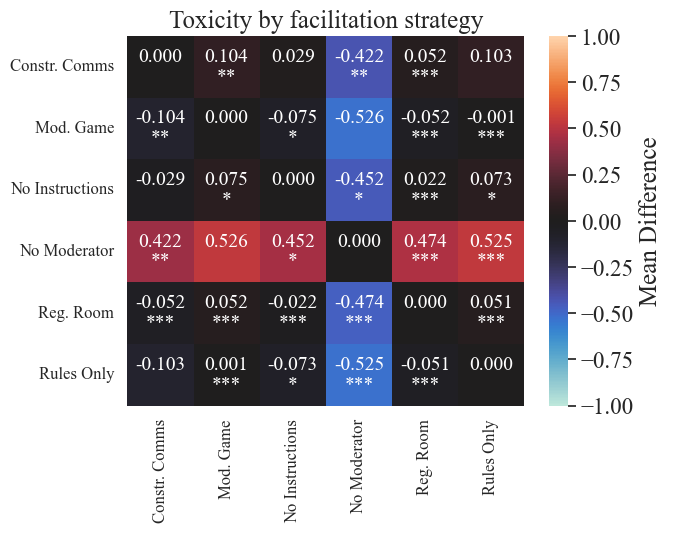
\includegraphics[width=\linewidth]{toxicity_stats.png}
	\centering
	\caption{Mean difference of Toxicity between pairs of facilitation strategies. When the value of a cell at row $i$ and column $j$ is $x$, strategy $i$ leads to overall more (worse) ($x>0$) toxicity, or less (better) ($x<0$) toxicity compared to $j$ for an average of $x$ points in a scale of $1-5$. For each comparison, we use a pairwise Student t-test; p-values are shown as asterisks (\asterisknote).}
	\label{fig:toxicity_stats}
\end{figure}

\paragraph{Sophisticated facilitation strategies dampen toxicity over time} Table~\ref{tab:toxicity} demonstrates that the average toxicity with \emph{\strategynomod} is $2.164$ (\emph{Intercept}). For each dialogue turn, toxicity drops by an average of $-0.012$ points (\emph{time}), while discussions following the \emph{\strategyregroom} strategy feature an average of  $-0.277$ (less) toxicity, and an additional $-0.023$ average drop per dialogue turn (\emph{\strategyregroom}$\times$\textit{time}). We note that our strategy (\emph{\strategymodgame}), the \emph{\strategyregroom}, and \emph{\strategyconstrcomm} strategies cause a statistically significant drop in toxicity over time.

\begin{table}[t]
	\centering
	\begin{tabular}{l p{2.5cm}}
		\toprule
		\textbf{Variable} & \textbf{Toxicity} \\
		\midrule
		Intercept & 2.164\textsuperscript{***} \\
		\strategynoinstr & -0.426\textsuperscript{***} \\
		\strategymodgame & -0.435\textsuperscript{***} \\
		\strategyrules & -0.461\textsuperscript{***} \\
		\strategyregroom & -0.277\textsuperscript{***} \\
		\strategyconstrcomm & -0.230\textsuperscript{***} \\
		time & -0.012\textsuperscript{**} \\
		\strategynoinstr$\times$time & -0.003 \\
		\strategymodgame$\times$time & -0.011\textsuperscript{*} \\
		\strategyrules$\times$time & -0.008 \\
		\strategyregroom$\times$time & -0.023\textsuperscript{***} \\
		\strategyconstrcomm$\times$time & -0.023\textsuperscript{***} \\
		\bottomrule
	\end{tabular}
	\small
	\asterisknote
	\normalsize
	\caption{\ac{OLS} regression coefficients for Toxicity ($Adj. R^2=0.054$). \textit{“Time”} denotes dialogue turn, reference factor is \emph{\strategynomod}.}
	\label{tab:toxicity}
\end{table}

\paragraph{Sophisticated facilitation strategies however do not qualitatively further improve synthetic discussions.} The impact of the \emph{\strategyrules}, \emph{\strategyregroom} and \emph{\strategyconstrcomm}  strategies (\S\ref{ssec:experimental:strategies}) is marginal, and sometimes even not statistically significant compared to the second baseline (\emph{\strategynoinstr}) (Fig.~\ref{fig:toxicity_stats}). This suggests that out-of-the-box \acp{LLM} may be unable to effectively use advanced instructions, verifying research pointing to important limitations in \ac{LLM} facilitators \cite{cho-etal-2024-language}.

\paragraph{\ac{LLM} facilitators choose to intervene far too frequently.} Fig.~\ref{fig:intervention_count} demonstrates that \ac{LLM} facilitators intervene at almost any opportunity, even though they are instructed to only do so when necessary. Additionally, a qualitative look through the dataset reveals that \ac{LLM} user-agents exhibit atypical tolerance for excessive facilitator interventions. Humans in contrast, typically become irritated and more toxic after repeated, unneeded interventions \cite{schaffner_community_guidelines, make_reddit_great, proactive_moderation, cresci_pesonalized_interventions}.

\begin{figure}[t]
	\centering
	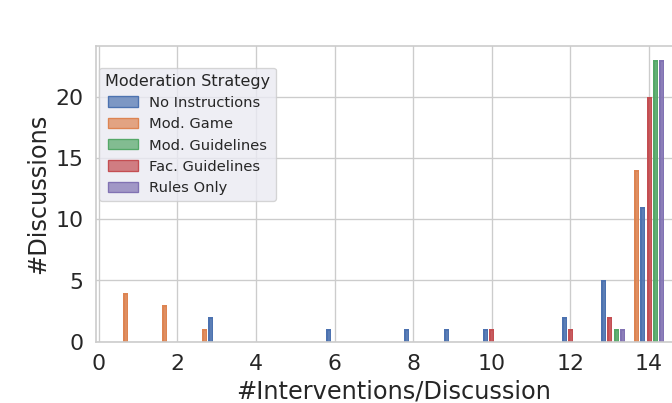
\includegraphics[width=\columnwidth]{intervention_count.png}
	\caption{Histogram of interventions by \ac{LLM} facilitators. The maximum number of interventions is $14$.}
	\label{fig:intervention_count}
\end{figure}

\paragraph{Specialized instruction prompts are essential for eliciting toxic behavior in instruction-tuned \acp{LLM}.} Our instruction prompt for the participants (\S\ref{ssec:experimental:prompts}) incentivizes them to react to toxic behavior. Indeed, discussions involving “Troll” user-agents, led to increased toxicity among \emph{other} participants, even under the \emph{\strategynoinstr} strategy (blue, bottom bars in Fig.~\ref{fig:toxicity_trolls}; Student's t-test $p < .000$). This effect diminishes when we remove these instructions (orange, top bars in Fig.~\ref{fig:toxicity_trolls}).

\begin{figure}[t]
    \centering
    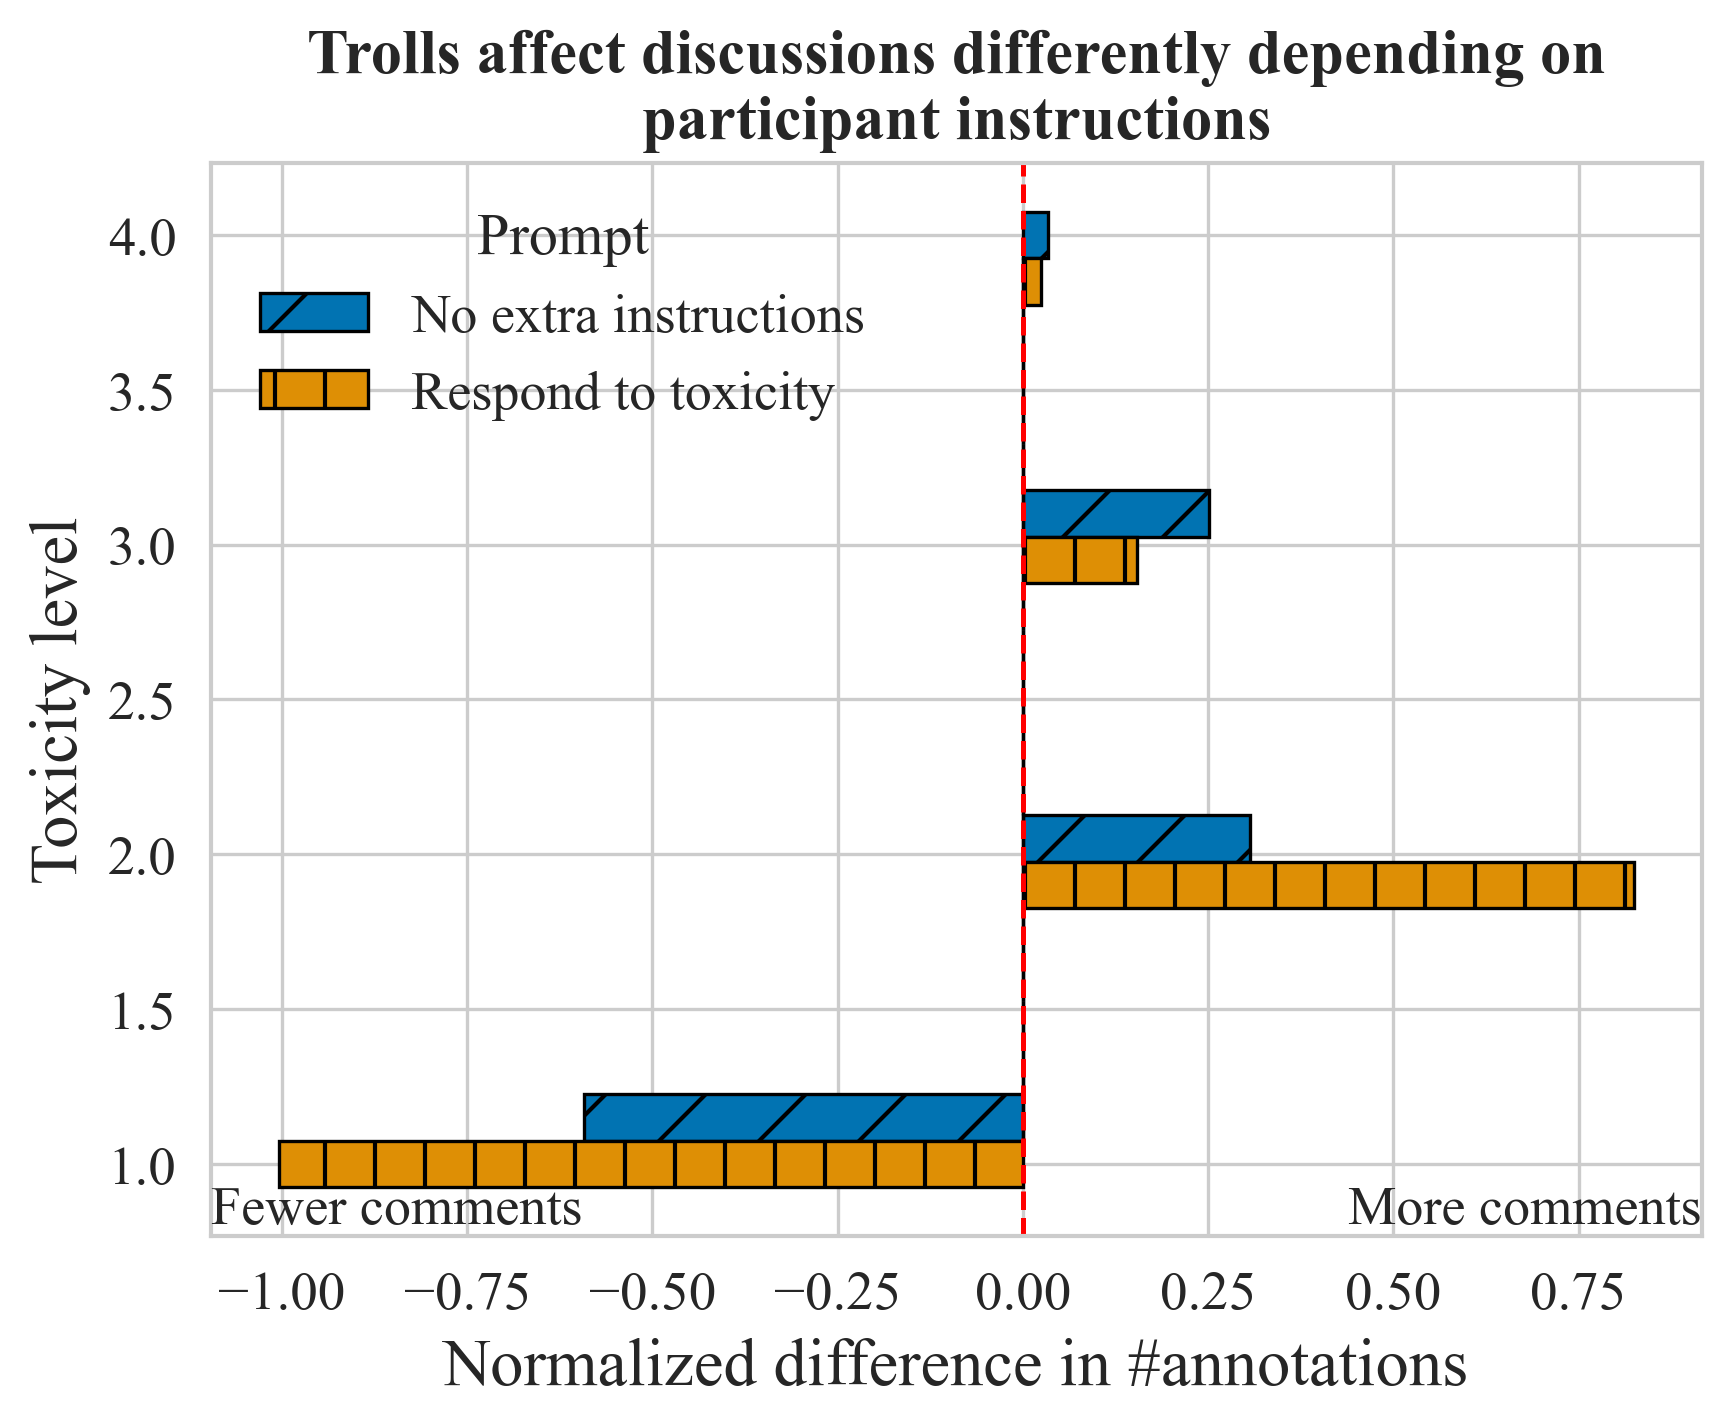
\includegraphics[width=0.8\linewidth]{toxicity_trolls.png}
    \caption{Relative differences in \#toxicity annotations of synthetic discussions. Bars extending to the right (left) of the line indicate more (less) annotations for discussions with no ``troll'' agents present compared to ones with ``trolls''.}
    \label{fig:toxicity_trolls}
\end{figure}


\subsection{Ablation Study}
\label{ssec:results:ablation}

\begin{figure*}[t]
    \begin{subfigure}{0.32\linewidth}
        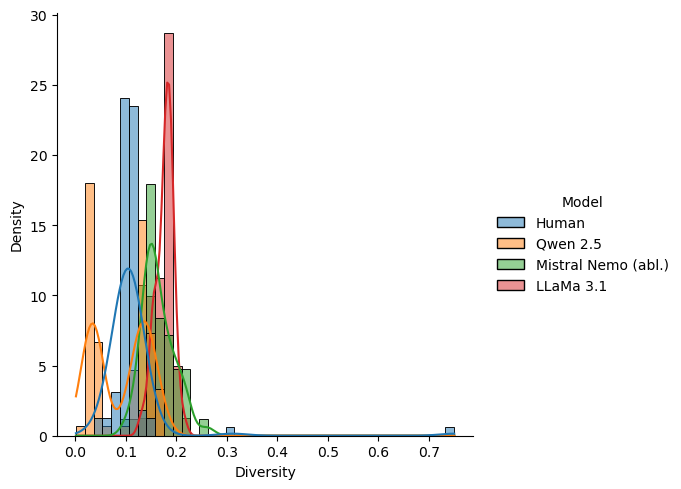
\includegraphics[width=\textwidth]{rougel_model.png}
        \caption{Model}
        \label{fig:rougel_model}
    \end{subfigure}%
    \hfill
    \begin{subfigure}{0.32\linewidth}
        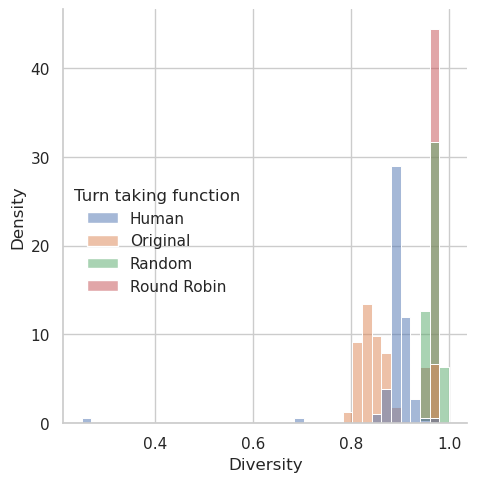
\includegraphics[width=\textwidth]{rougel_turns.png}
        \caption{Turn-taking function $t$}
        \label{fig:rougel_turns}
    \end{subfigure}%
    \hfill
    \begin{subfigure}{0.32\linewidth}
        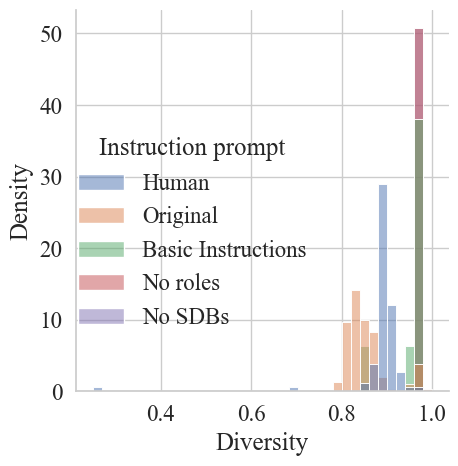
\includegraphics[width=\textwidth]{rougel_prompts.png}
        \caption{Promoting function $\phi$}
        \label{fig:rougel_prompts}
    \end{subfigure}%

    \caption{Diversity (\S\ref{ssec:related:quality}) distribution for each discussion by \ac{LLM} (\S\ref{ssec:experimental:setup}), turn-taking function $t$ (\S\ref{ssec:experimental:turn}), and prompting function $\phi$ used (\S\ref{ssec:experimental:prompts}).}
    \label{fig:diversity}
\end{figure*}

\begin{figure*}[t]
    \begin{subfigure}{0.32\linewidth}
        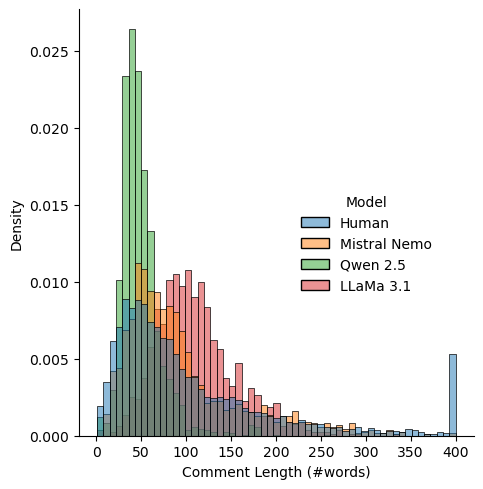
\includegraphics[width=\textwidth]{comment_len_model.png}
        \caption{Model}
        \label{fig:comment_length_model}
    \end{subfigure}%
    \hfill
    \begin{subfigure}{0.32\linewidth}
        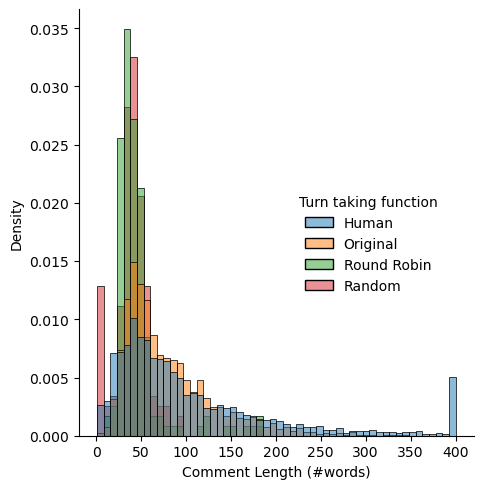
\includegraphics[width=\textwidth]{comment_len_turns.png}
        \caption{Turn-taking function $t$}
        \label{fig:comment_length_turns}
    \end{subfigure}%
    \hfill
    \begin{subfigure}{0.32\linewidth}
        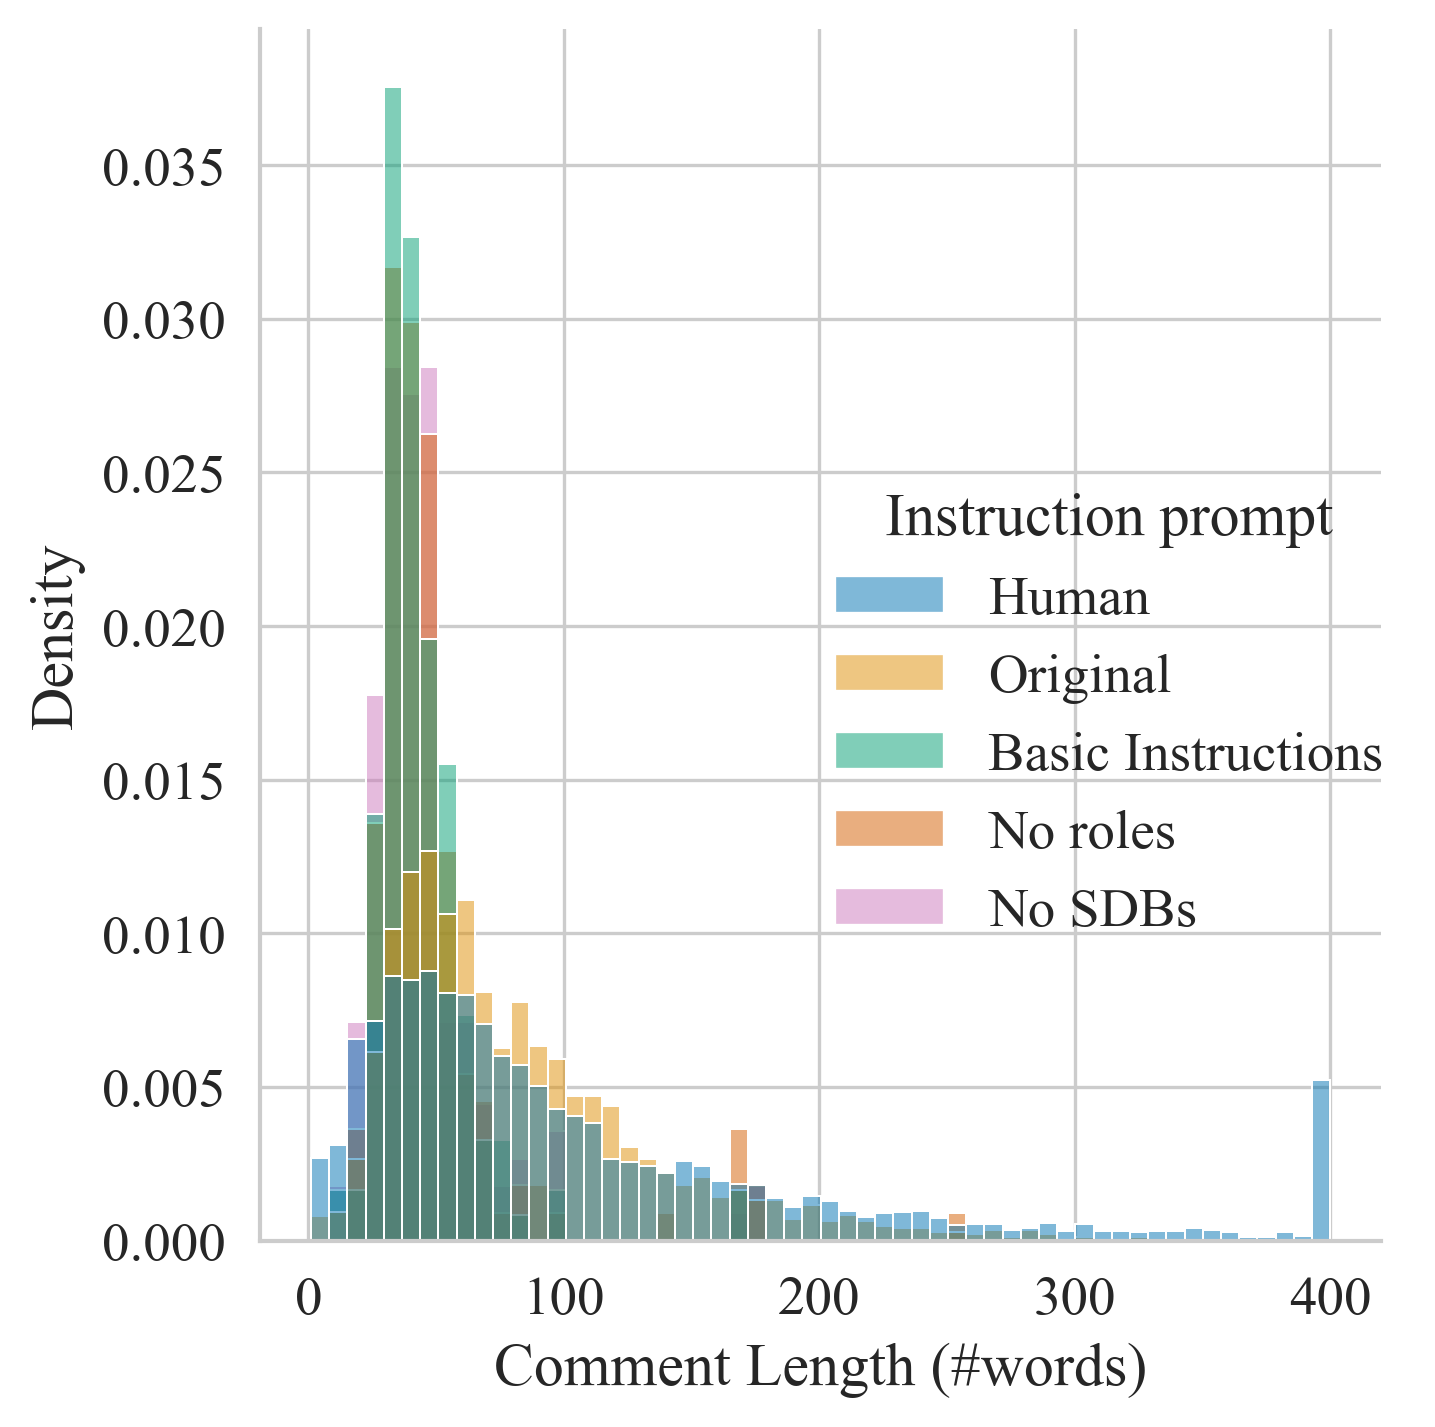
\includegraphics[width=\textwidth]{comment_len_prompts.png}
        \caption{Prompting function $\phi$}
        \label{fig:comment_length_prompts}
    \end{subfigure}%

    \caption{Comment length for each discussion by \ac{LLM} (\S\ref{ssec:experimental:setup}), turn-taking function $t$ (\S\ref{ssec:experimental:turn}), and prompting function $\phi$ used (\S\ref{ssec:experimental:prompts}). For ease of comparison, comments above 400 words are marked at the end of the x-axis.}
    \label{fig:comment_length}
\end{figure*}


We generated eight synthetic discussions per ablation experiment, using a single model, Qwen, to limit computational cost. We evaluated the diversity (cf. \S\ref{ssec:related:quality}) of the ablated discussions by comparing them with: (1) discussions in our original dataset produced solely by the Qwen model; and (2) human discussions from the \ac{CeRI} “Regulation Room” dataset\footnote{\url{http://archive.regulationroom.org}. Disclaimer: Any opinions, findings, and conclusions or recommendations expressed in this material are those of the author(s) and do not necessarily reflect the views of the \ac{CeRI}.}, which includes moderated online deliberative discussions for ten diverse topics.


\subsubsection{Effects of LLMs}

\paragraph{Mistral and Qwen generate discussions more aligned with human diversity scores, despite being significantly smaller than the LLaMa model.} As is shown in Fig.~\ref{fig:rougel_model}, Qwen demonstrated the highest diversity among the evaluated models, indicating limited participant interaction (\S\ref{ssec:related:quality}), followed by Mistral Nemo and LLaMa. However, none of the models closely matched the diversity observed in human discussions. 
LLaMa's lower diversity validates prior research suggesting that highly aligned \acp{LLM} struggle to replicate human dynamics \cite{Park2023GenerativeAI, leng_2024}. Alternatively, it can be partially attributed to its longer average comment length (Fig.~\ref{fig:comment_length_model}); we find that there is a statistically significant, negative correlation between comment length and diversity in synthetic discussions (Student's t-test  $p < .000$), although we can not verify this pattern in human-generated texts ($p = 0.775$).


\subsubsection{Effects of Turn-Taking Functions}

\paragraph{Our proposed turn-taking function meaningfully improves the quality of synthetic data.} We compare our turn-taking function (\S\ref{ssec:experimental:turn}) to two baselines: Round Robin (participants speaking one after the other, then repeating) and Random Selection (uniformly sampling another participant each turn). Fig.~\ref{fig:rougel_turns} demonstrates that no single function fully approximates human diversity scores (all distributions diverge from the blue—human—distribution). However, unlike our own function, both baselines feature extremely high diversity, which can not be attributed to lengthier comments (Fig.~\ref{fig:comment_length_turns}). Additionally, comments following our turn-taking function, closely follow the length of human discussions (Fig.~\ref{fig:comment_length_turns}).


\subsubsection{Effects of User Prompting}

We conduct three separate experiments in which user-agents (excluding facilitators) are subjected to one of the following conditions at a time: (1) no assigned \acp{SDB}, (2) no assigned roles, or (3) only a basic instruction prompt given (\S\ref{sssec:appendix:actors}). 

\paragraph{\acp{SDB}, roles and our instruction prompt increase the quality of synthetic data.} Fig.~\ref{fig:rougel_prompts} illustrates that although our proposed methodology---incorporating \acp{SDB}, roles, and specialized instruction prompts---does not achieve discussions with diversity scores comparable to human ones, replacing any of the above results in a notable deterioration. For instance, omitting \acp{SDB} (denoted as ``No \acp{SDB}'' and represented by the red distribution in Fig.~\ref{fig:rougel_prompts}) causes the majority of discussions to exhibit maximum diversity---one---indicating a significant loss in participant interaction, which is not caused by longer comment length (Fig.~\ref{fig:comment_length_prompts}). This decline is analogous to the effects observed when modifying the turn-taking function. Also similarly to the turn-taking ablation study, our proposed methodology w.r.t. prompts, features comments that best emulate observed human comment length (Fig.~\ref{fig:comment_length_prompts}).